\chapter{Testing mit \emph{DeepEval}}
\label{chap:testing}

\section{Framework/Deepeval}

Die Wahl des Frameworks fiel auf Deepeval, da Deepeval die genaue Überprüfung der gesamten RAG-Pipeline in verschiedensten Systemen ermöglicht. DeepEval ist ein opensource  Python Framework speziell dafür entwickelt LLM Applikationen zu evaluieren. Hierfür können verschiedenste LLMs als Judge-Modelle genutzt werden, die basierend auf vorher definierten Metriken die Qualität der Antworten und Chunks bewerten. Außerdem ermöglicht Deepeval die native Integration durch Pytest, sowie multi-modale Evaluation und die automatische Optimierung von Prompts. Im Kontext des Chatbots bot sich die End-To-End LLM Evaluation von DeepEval an, da es sich um eine relativ simple Architektur handelt und die Anfragen nur Fragen und Anworten sind, die durch einen einzigen LLM-Testcase repräsentiert bzw. getestet werden können.

Hierbei wird eine einzelne Testinstanz über einen LLMTestCase abgebildet, welcher die Eingabe-Query, Ausgabe und den Retrieval-Kontext beinhaltet. Als Judge Modell stehen in dem Projekt zwei Implementationen bereit. Hierbei kann der Nutzer zwischen OpenAI und AWS Bedrock unterscheiden und die entsprechenden Modelle selbst auswählen. In den meisten Tests wurde das OpenAI Modell GPT-4o-mini genutzt. Es kann außerdem zwischen verschiedenen Metriken ausgewählt werden, welche daraufhin in jedem einzelnen Testfall geprüft werden und anhand eines  vorher definierten Threshhold Wertes von 0.0-1-0 kann definiert werden, ob ein Test fehlschägt oder erfolgreich ist.

\section{Überblick}
Der Aufbau ist in Abbildung \ref{fig:e2e} zu sehen.
\begin{figure}[h] 
    \centering
    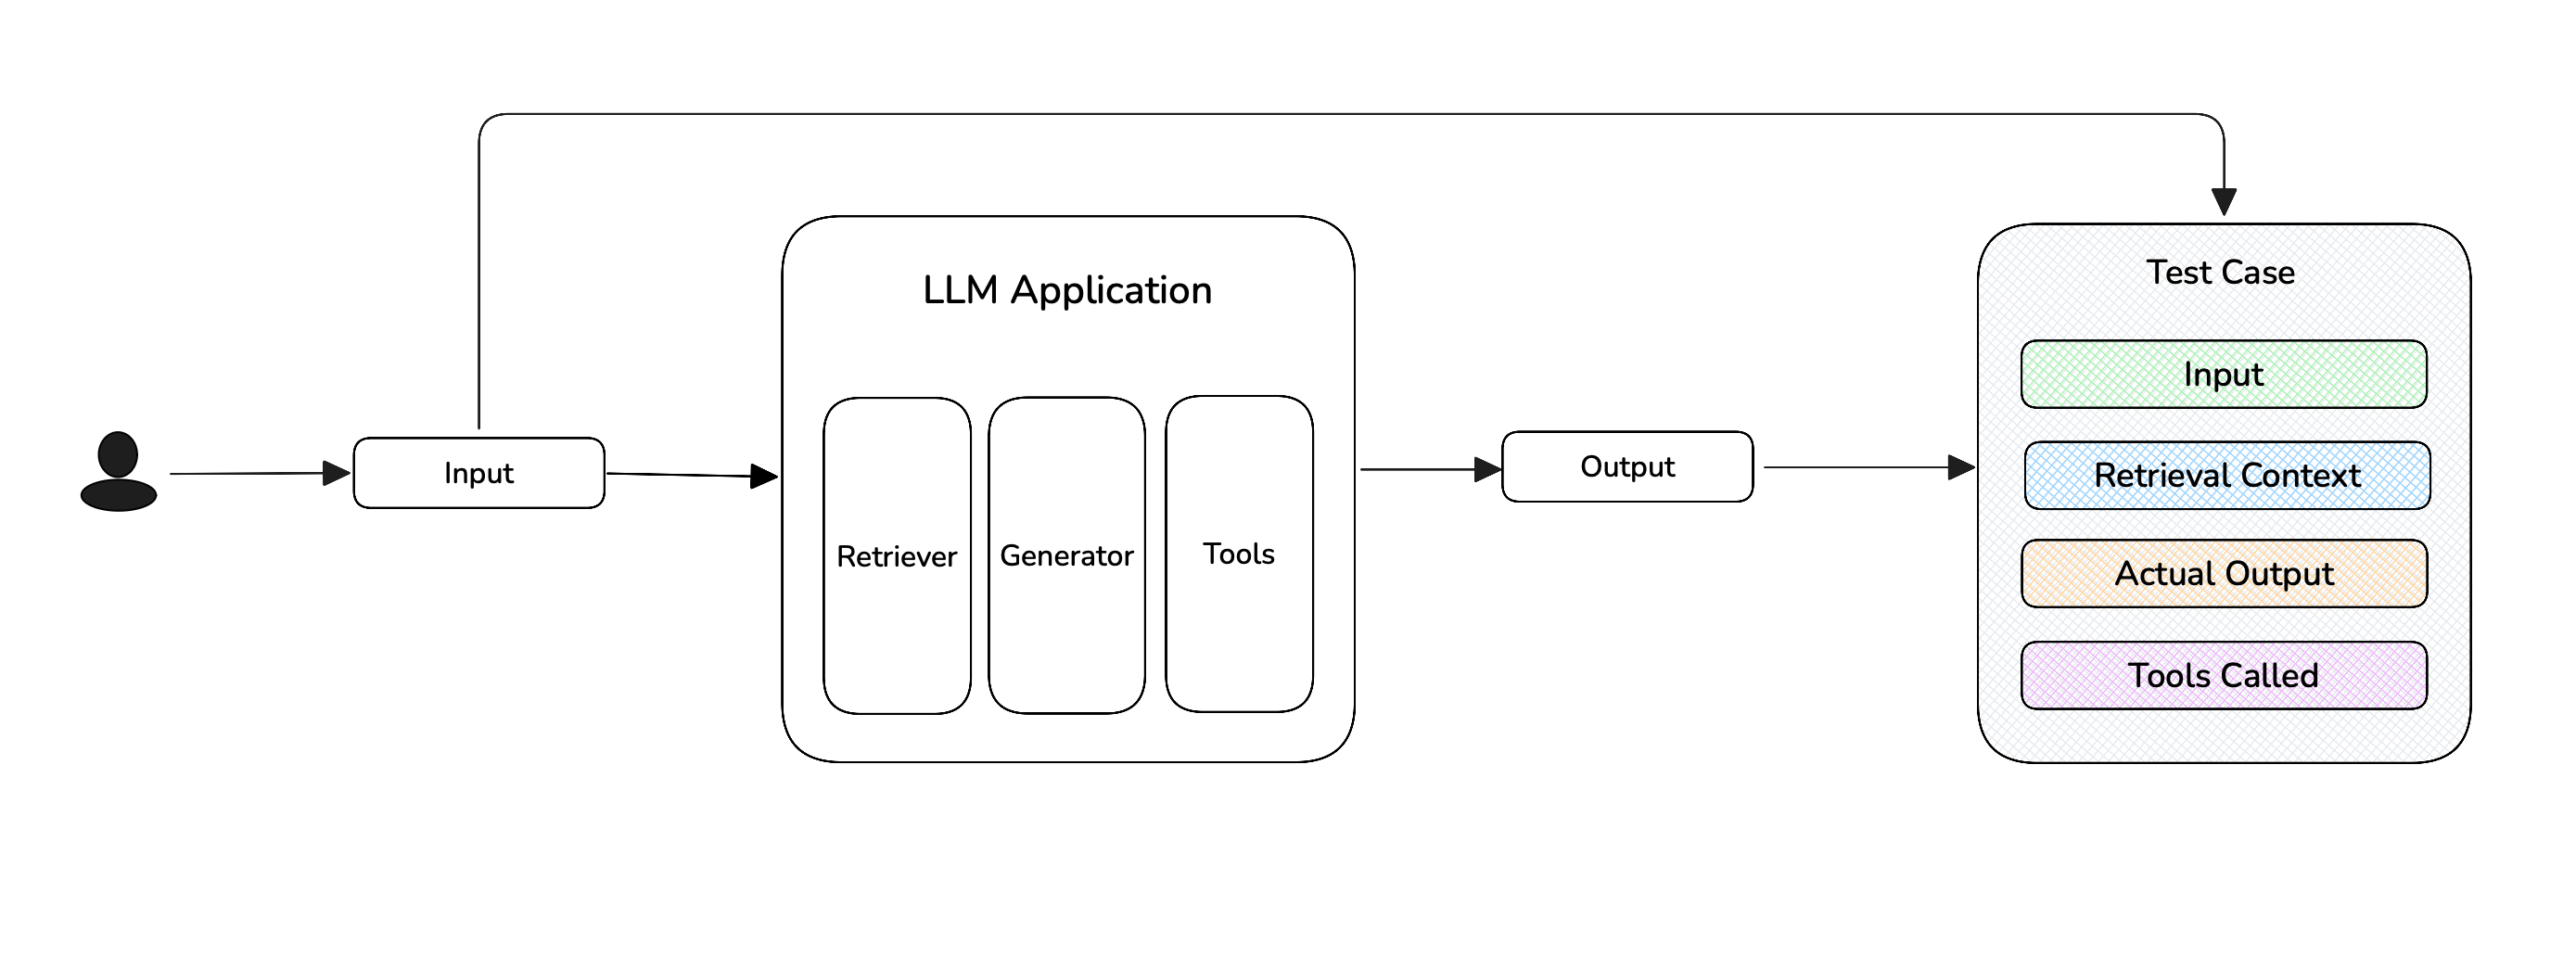
\includegraphics[width=0.8\textwidth]{bilder/e2e}\\
    \caption{End-To-End Evaluation}
    \label{fig:e2e}
\end{figure}

Hierbei wird die RAG-Pipeline als Blackbox behandelt und es werden nur die Eingaben und Ausgaben, sowie die benutzten Tools evaluiert.

Um einen Testdurchlauf zu starten kann der Nutzer einfach den Test Runner ausführen, welcher die gesamte RAG-Pipeline für jede der vordefinierten Queries durchläuft. Hierbei werden die retrieved Chunks und die Antwort gespeichert und anhand der Metriken bewertet.


\section{Metriken}
Wir haben uns in dem Projekt für die drei Metriken AnswerRelevancy, Faithfulness und ContextualRelevancy entschieden, um die wichtigsten Bereiche abzudecken und zu überprüfen.

\subsubsection{AnswerRelevancy}
Hierbei geht es darum zu identifizieren, ob die generierte Antwort relevant für die gestellte Frage ist. Es wird evaluiert, ob die Antwort tatsächlich das gefragte addressiert oder nicht und bewertet Antworten schlechter, die nicht zum Thema passen oder zu ungenau sind. Hierbei wird jedoch nicht geprüft, ob die Antworten faktisch korrekt sind. Der Threshhold ist hierbei 0.5 und eine beispielhafte, fehlerhatfe Anwort könnte so aussehen:

Query: \enquote{Wie viel ECTS hat Digitaltechnik?}\newline
Answer: \enquote{Die FH Wedel bietet viele Module an...} → Fails (doesn't answer question)

\subsubsection{Faithfulness}
Diese Metrik bezieht sich auf die generierten Chunks aus dem Retrieval Kontext. Hierbei wird überprüft, ob die generierte Antwort und jede einzelne Aussage auf den Chunks basiert. Das ist vorallem wichtig für die Halluzinationserkennung und essenziell für die Vertrauenswürdigkeit des Chatbots. Der Threshhold ist hierbei 0.5 und eine beispielhafte, fehlerhatfe Anwort könnte so aussehen:

Retrieved chunks mention \enquote{7 Semester Regelstudienzeit}\newline
Answer says \enquote{6 Semester} → Fails (hallucination)

\subsubsection{ContectRelevancy}
Diese Metrik bewertet die Relevanz und Qualität der Chunks bezüglich der Frage. Hierbei wird also der Retrieval-Prozess evaluiert und nicht die generierte Antwort. Der Threshhold ist hierbei nur  0.25, weil chunks oft extra Kontext beinhalten und eine beispielhafte, fehlerhatfe Anwort könnte so aussehen:

Query: \enquote{Prüfungsordnung Bachelor Informatik}\newline
Retrieved chunks: Curriculum tables, module descriptions → Fails (wrong doc types)

\section{Judge Models}
Anfangs wurde der Ansatz lokale Modelle für die Evaluierung zu nutzen verfolgt, um Kosten zu sparen und Datensicherheit zu gewährleisten, allerdings stießen wir hier auf einige Probleme. Das Hauptproblem war die Qualität der Evaluierung durch kleinere, lokale Modelle mit bis zu 7B Parametern. Diese Modelle sind zu klein, um richtige Bewertungen  vorzunehmen und gaben außerdem sehr stark variierende Bewertungen bei den gleichen Fragen. Außerdem war die benötigte Zeit um ein vielfaches höher als über die entsprechenden API-Anfragen.

Deshalb fiel die Wahl dann auf die vorgesehende Nutzung von DeepEval über API-Anfragen an Judge Modelle verschiedenster Anbieter. Hierbei haben wir uns für OpenAI und AWS Bedrock entschieden, um so viele Modelle wie möglich testen zu können. Die jetzige Implementation nutzt  das OpenAI Modell GPT-4o-mini als Judge, weil die Bedrock Tokens nach ungefähr 12 Stunden ablaufen und erneuert werden müssen, was im laufenden Betrieb ungeeignet ist. Dadurch sind die Anfragen schnell und verlässlich und die Evaluationsqualität ist konstistent, während die Kosten der Anfragen überschaubar bleiben. Als Fallback dient der Bedrock Judge, welcher bei fehlschlagenden OpenAI Anfragen oder ausgefallenem Service übernimmt. Hierbei stehen verschiedene Modelle zur Verfügung wie z.B:

\begin{table}[htbp]
\centering
\begin{tabular}{|l|l|l|}
\hline
\textbf{Modell} & \textbf{Anfrageformat} & \textbf{Hinweise} \\
\hline
anthropic.claude-* & Messages API & Beste Qualität \\
amazon.titan-* & inputText & Schnell \\
meta.llama* & prompt & Offene Gewichte \\
amazon.nova-* & Messages mit Content-Array & AWS-nativ \\
\hline
\end{tabular}
\caption{Unterstützte Modelle}
\end{table}

\section{Testinfrastruktur}
Die Hauptklasse der Tests gliedert sich in die Wahl des Evaluationsmodells, die Auswahl der Metriken und Threshholds, die Deklaration der Tests und hat folgenden Aufbau:

\begin{lstlisting}[language=Python, caption={test-rag-quality Klasse}]
# 1. Load environment variables
load_dotenv(op.join(_RAG_ROOT, ".env"), override=True)

# 2. Select judge (OpenAI preferred, Bedrock fallback)
if _OPENAI_KEY.startswith("sk-"):
    _judge_model = get_openai_judge()
else:
    _judge_model = get_bedrock_judge()

# 3. Configure metrics with thresholds
answer_rel = AnswerRelevancyMetric(threshold=0.5, model=_judge_model)
faithful = FaithfulnessMetric(threshold=0.5, model=_judge_model)
ctx_rel = ContextualRelevancyMetric(threshold=0.25, model=_judge_model)

# 4. Parameterized test function
@pytest.mark.parametrize("query", [...])
def test_rag_quality(query):
    answer, retrieval_context = run_single_turn(query)
    test_case = LLMTestCase(
        input=query,
        actual_output=answer,
        retrieval_context=retrieval_context,
    )
    assert_test(test_case, [answer_rel, faithful, ctx_rel])
\end{lstlisting}

Die zweite relevante Klasse ist die Adapter Klasse, die das Test-Framework und die RAG-Pipeline wie folgt kombiniert:
\begin{lstlisting}[language=Python, caption={Eval-Adapter Klasse}]
def run_single_turn(query: str) -> Tuple[str, List[str]]:
    # 1. Context detection (degree, program, doctype)
    context_state = detect_context(query, context_state)
    
    # 2. Query expansion with LLM
    expanded_query, original_query, keywords = expand_query_with_llm(...)
    
    # 3. Hybrid retrieval (semantic + keyword)
    documents = hybrid_search(expanded_query, top_k=TOP_K * 2)
    
    # 4. Reranking with metadata boost
    documents = rerank_with_metadata_boost(original_query, documents, top_k=TOP_K)
    
    # 5. Generate answer
    generator = OpenAIGenerator(api_base_url=None)
    answer = generator.run(prompt=prompt)
    
    # 6. Return answer and chunk contents
    return answer, [doc.content for doc in documents]
\end{lstlisting}

Außerdem stehen weitere Debug Methoden zur Verfügung um einzlene Komponenten wie den Retrieval Prozess separat zu testen, ohne die gesamte Testsuite auszuführen. Hierbei werden der Documentstore status, Ergebnisse von Keyword und semantischer Suche, sowie Hybride Suchergebnisse überprüft und ausgegeben.
\section{Ausführung}

Die Ausführung funktioniert wie folgt:

\begin{lstlisting}[language=Python, caption={Ausführung der Tests}]
cd rag-code

# Run all tests (verbose)
python -m pytest tests/test_rag_quality.py -v

# Filter by keyword
python -m pytest tests/test_rag_quality.py -v -k "Informatik"

# With DeepEval dashboard (web UI)
python -m deepeval test run tests/test_rag_quality.py

# Single test only
python -m pytest tests/test_rag_quality.py -v -k "regelstudienzeit"
\end{lstlisting}
Nach der Ausführung hat das Ergebnis die folgende Form in der Konsole:


QUERY: Was ist die regelstudienzeit im Bachelor Informatik?

ANSWER: Die Regelstudienzeit beträgt 7 Semester...

Retrieved 10 chunks:\newline
  [1] Kontext: Studienabschluss: Bachelor, Studiengang: Informatik...\newline
  [2] Prüfungsordnung Informatik (Bachelor) an der FH Wedel...\newline
PASSED / FAILED

Hierbei ist gut zu erkennen welche Tests fehlgeschlagen sind und warum.

\section{Testfragen}
Die Testfragen unterscheiden sich in normale Fragen und Vergleichsfragen. Wir haben die folgenden Fragen so gewählt, um ein möglichst breites Spektrum abzudecken und mögliche Probleme gut einordnen zu können.

\begin{figure}[h] 
    \centering
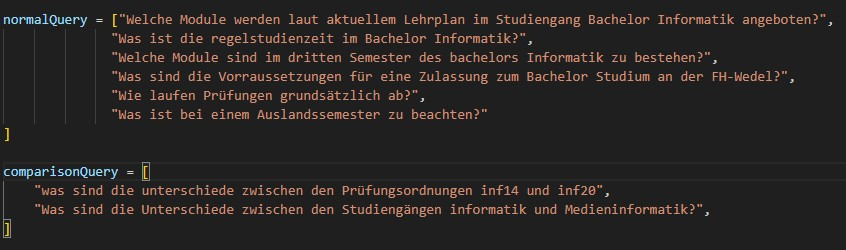
\includegraphics[width=1.0\textwidth]{bilder/queries}\\
    \caption{End-To-End Evaluation}
    \label{fig:e2e}
\end{figure}

\section{Ergebnisse}
Die Metriken liefern jeweils Punkte von 0 bis 1, wobei die Qualität in 0.25 Schritten gemessen wird. DeepEval erlaubt das include-reason Flag zu setzen und somit die Gründe für die Bewertung mit auszugeben was so aussehen kann:

AssertionError: Metrics: Answer Relevancy (score: 0.0, threshold: 0.5, 
reason: The response completely fails to address the question about 
the ECTS credits for the module Digitaltechnik...)

Während der Tests fielen einige Muster auf, die auf verschiedene Probleme hinwiesen, welche in der Folge direkt behoben werden konnten.

\begin{table}[htbp]
\centering
\begin{tabular}{|l|l|l|}
\hline
\textbf{Muster} & \textbf{Wahrscheinliche Ursache} & \textbf{Lösung} \\
\hline
Answer Relevancy = 0 & LLM liefert keine Antwort & Retrieval verbessern \\
Faithfulness = 0 & LLM halluziniert & Prompt anpassen \\
Contextual Relevancy = 0 & Retrieval Probleme & Parser/Metadaten korrigieren \\
Alle Metriken niedrig & Leeres Retrieval & Qdrant Daten überprüfen \\
\hline
\end{tabular}
\caption{Fehlermuster und Gegenmaßnahmen}
\end{table}


Allgemein geben die Tests Aufschluss darauf was gut funktioniert und wo noch Verbesserungspotential besteht. Fragen zu Prüfungsordnungen bzw.  zu allen PVO, ZLO und SPO ergeben in den meisten Fällen gute Ergebnisse und werden gut bewertet. Auch Modulspezifische Fragen werden korrekt beantwortet, indem das gesuchte Modul und der Studiengang herausgefunden werden und die korrekten Chunks abgerufen werden. Fragen zu Modulübersichten, Faktenfragen, Zulassungsfragen, Prüfungsfragen und Fragen zu allgemeinen Regelungen beantwortet der Chatbot mit einer sehr hohen Erfolgsrate. Besonders die MEtriken AnswerRelevancy und Faithfulness werden in den meisten Fällen bestanden. und auch die Antwortzeiten sind vielversprechend.

Verbesserungspotential besteht bei Vergleichen zwischen Modulen, sowie versionsspezifische Fragen. Hier müssten die Parser noch verfeinert werden, um die genauen Versionen und Dokumenttypen herauszufinden, aber im allgemeinen sind die generierten Antworten des Chatbots gut und für sehr spezifische Fragen können in der Zukunft eigene Tools in den Prozess integriert werden, um die Genauigkeit zu verbessern. Die Metrik bezüglich der Kontextuellen Relevanz der abgerufenen Chunks schlägt noch relativ häufig fehl, da zu viele irrelevante Chunks in den TOP-K Chunks sind, allerdings ist der Threshhol dieser Metrik auch nur 0.25 und könnte angepasst werden. Die generierten Antworten sind hierbei oft korrekt, allerdings sorgt der hohe Kontextuelle \enquote{Lärm} für ein Fehlschlagen der Tests.


